\documentclass[xcolor=dvipsnames]{beamer}
\usepackage{Sweave}
\usepackage{booktabs}
\usepackage{float}
\usepackage{booktabs}
\usepackage{amssymb}
\usepackage{amsmath}
\usepackage{float}
\usepackage{xcolor}
\usepackage[english]{babel}
\usepackage{tikz}
\usepackage{listings}
\usepackage{amsmath,amssymb}
%\usecolortheme{dove}
%\usecolortheme{rose}
\definecolor{links}{HTML}{2A1B81}
\hypersetup{colorlinks,linkcolor=,urlcolor=links}
\restylefloat{table}
%\usetheme{Frankfurt}
\usetheme{Singapore}

%\usetheme{Pittsburgh}
\usecolortheme[named=blue]{structure}

\begin{document}
\Sconcordance{concordance:Reproducible_Research.tex:Reproducible_Research.Rnw:%
1 157 1}


\title{\textbf{Reproducible Research in R and \LaTeX}}

\titlepage{}

\begin{frame}{Reproducible Research}

...refers to the idea that the ultimate product of research is the paper with the full computational environment used to produce the results in the paper such as the data, code and these can be used to reproduce the results.

\vspace{7 mm}
\href{www.bepress.com/bioconductor/paper2/}{A paper by Robert Gentleman and Duncan Temple Lang}
\url{www.reproducibleresearch.org}\\
\href{www.econ.uiuc.edu/~roger/repro.html}{a web site by Roger Koenker}

\end{frame}

\begin{frame}{Literate programming}
Literate programming means that text, data, and computer code
are interwoven in a single self-contained document.

\end{frame}

\begin{frame}{What we are used to}
A research document involving multiple files with figures and tables
cut and paste from various places. For instance,

\begin{itemize}
\item a statistical software e.g stata do-file 
\item an excel spreadsheet with results
\item an excel spreadsheet with data
\item a directory with filenames like $“old.doc”$ and $“new.doc”$
\item a word document with tables and figures cut and paste from
various places
\end{itemize}

*Changes to the stata do-file are not automatically propogated to
the excel spread-sheet or to the Word document.

\end{frame}

\begin{frame}{Benefits of Literate Programming}

Integration of analysis and reporting
\begin{itemize}
\item No transcription errors
\item Automatic updating of results. i.e dynamic reports
\item Reproducible results

\end{itemize}

\end{frame}

\begin{frame}{Benefits of \LaTeX }


\begin{itemize}
\item Widespread use by the R community
\item Produces aesthetically beautiful documents
\item You don't have to worry about layout, it's all automatic.
\item Free
\item Scientific features like the references are available in \LaTeX.

\end{itemize}

\textbf{\colorbox{orange}{\textcolor{blue}{Disadvantage:}}}

Fairly steep learning curve

\end{frame}



\begin{frame}{Intergrating R and \LaTeX  with Sweave}
\textbf{\colorbox{orange}{\textcolor{blue}{Sweave}}}
\begin{itemize}
\item An R package written by Friedrich Leisch
\item Included with the base distribution of R
\item Supports integration of R with \LaTeX
\end{itemize}
\end{frame}

\begin{frame}{What does Sweave do?}
Essentially requires a single source document $– a ’.Rnw’ file.$
\centering
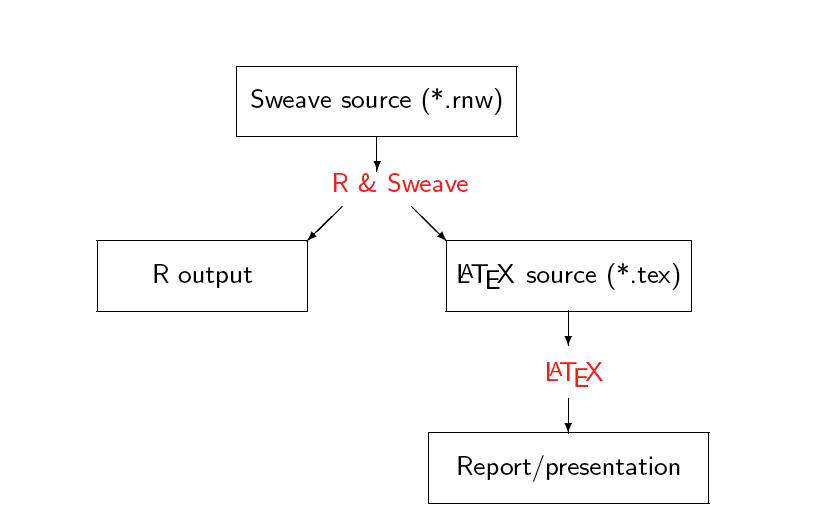
\includegraphics[width=10cm, height=7cm]{plot.png} 
\end{frame}


\begin{frame}{What does it Work?}
\begin{enumerate}
\item Write the LATEX file, but with extension .Rnw (or .Snw) instead of .tex:e.g \textcolor{red}{myfile.Rnw.}
\item The file will also contain  R code segments, suitably separated from the LATEX segments. 
 \item Within R, execute Sweave("myfile.Rnw"), assuming myfile.Rnw is in the working directory
of R.
\item This executes the code segments and will produce the file myfile.tex. 
\item  Run LATEX on ("myfile.tex") and obtain your report. 
\end{enumerate}

\end{frame}


\begin{frame}{What you need}

\begin{itemize}

\item A \LaTeX distribution (e.g., MiKTeX)
\item An editor configured for use with R and \LaTeX (E.g., R-Studio, Tinn-R,LyX, Kile) 
\item Instructions that are comprehensive but limited in scope.


\end{itemize}


\end{frame}




\begin{frame}[fragile]{\textbf{Resources}}

\setkeys{Gin}{width=0.62\linewidth}


\href{http://en.wikibooks.org/wiki/LaTeX/Introduction}{Introduction to LaTeX} \\
\href{http://www.stat.umn.edu/~charlie/Sweave}{A Sweave demo} \\
\href{http://www.ci.tuwien.ac.at/~leisch/Sweave}{Sweave and beyond}\\
\href{http://www.uncg.edu/cmp/reu/presentations/Charles%20Batts%20-%20Beamer%20Tutorial.pdf}{Beamer tutorial}

\end{frame}


\end{document}
